\subsection{Final Design}\label{subsec:final-design}

For the final design, the group went back to the hi-fi prototype and made some changes.
The group took into consideration their target audience when designing the user interface.
The interface is minimalistic, and the colors are simple to appeal to the co-workers at the café are mostly young
adults.
For gradient transitions, the group is using shades of blue, with darker shades representing higher values and lighter
shades representing lower values.
Blue was chosen as it contrasts well with its shades, which makes it easy to read the charts.
One requested change for the dashboard was to show more charts at the same time.
This was done by making the charts smaller and adding charts below each other.
These changes can be seen in Figure~\ref{fig:design-final-dash1} and Figure~\ref{fig:design-final-dash2}.

\begin{figure}[H]
    \centering
    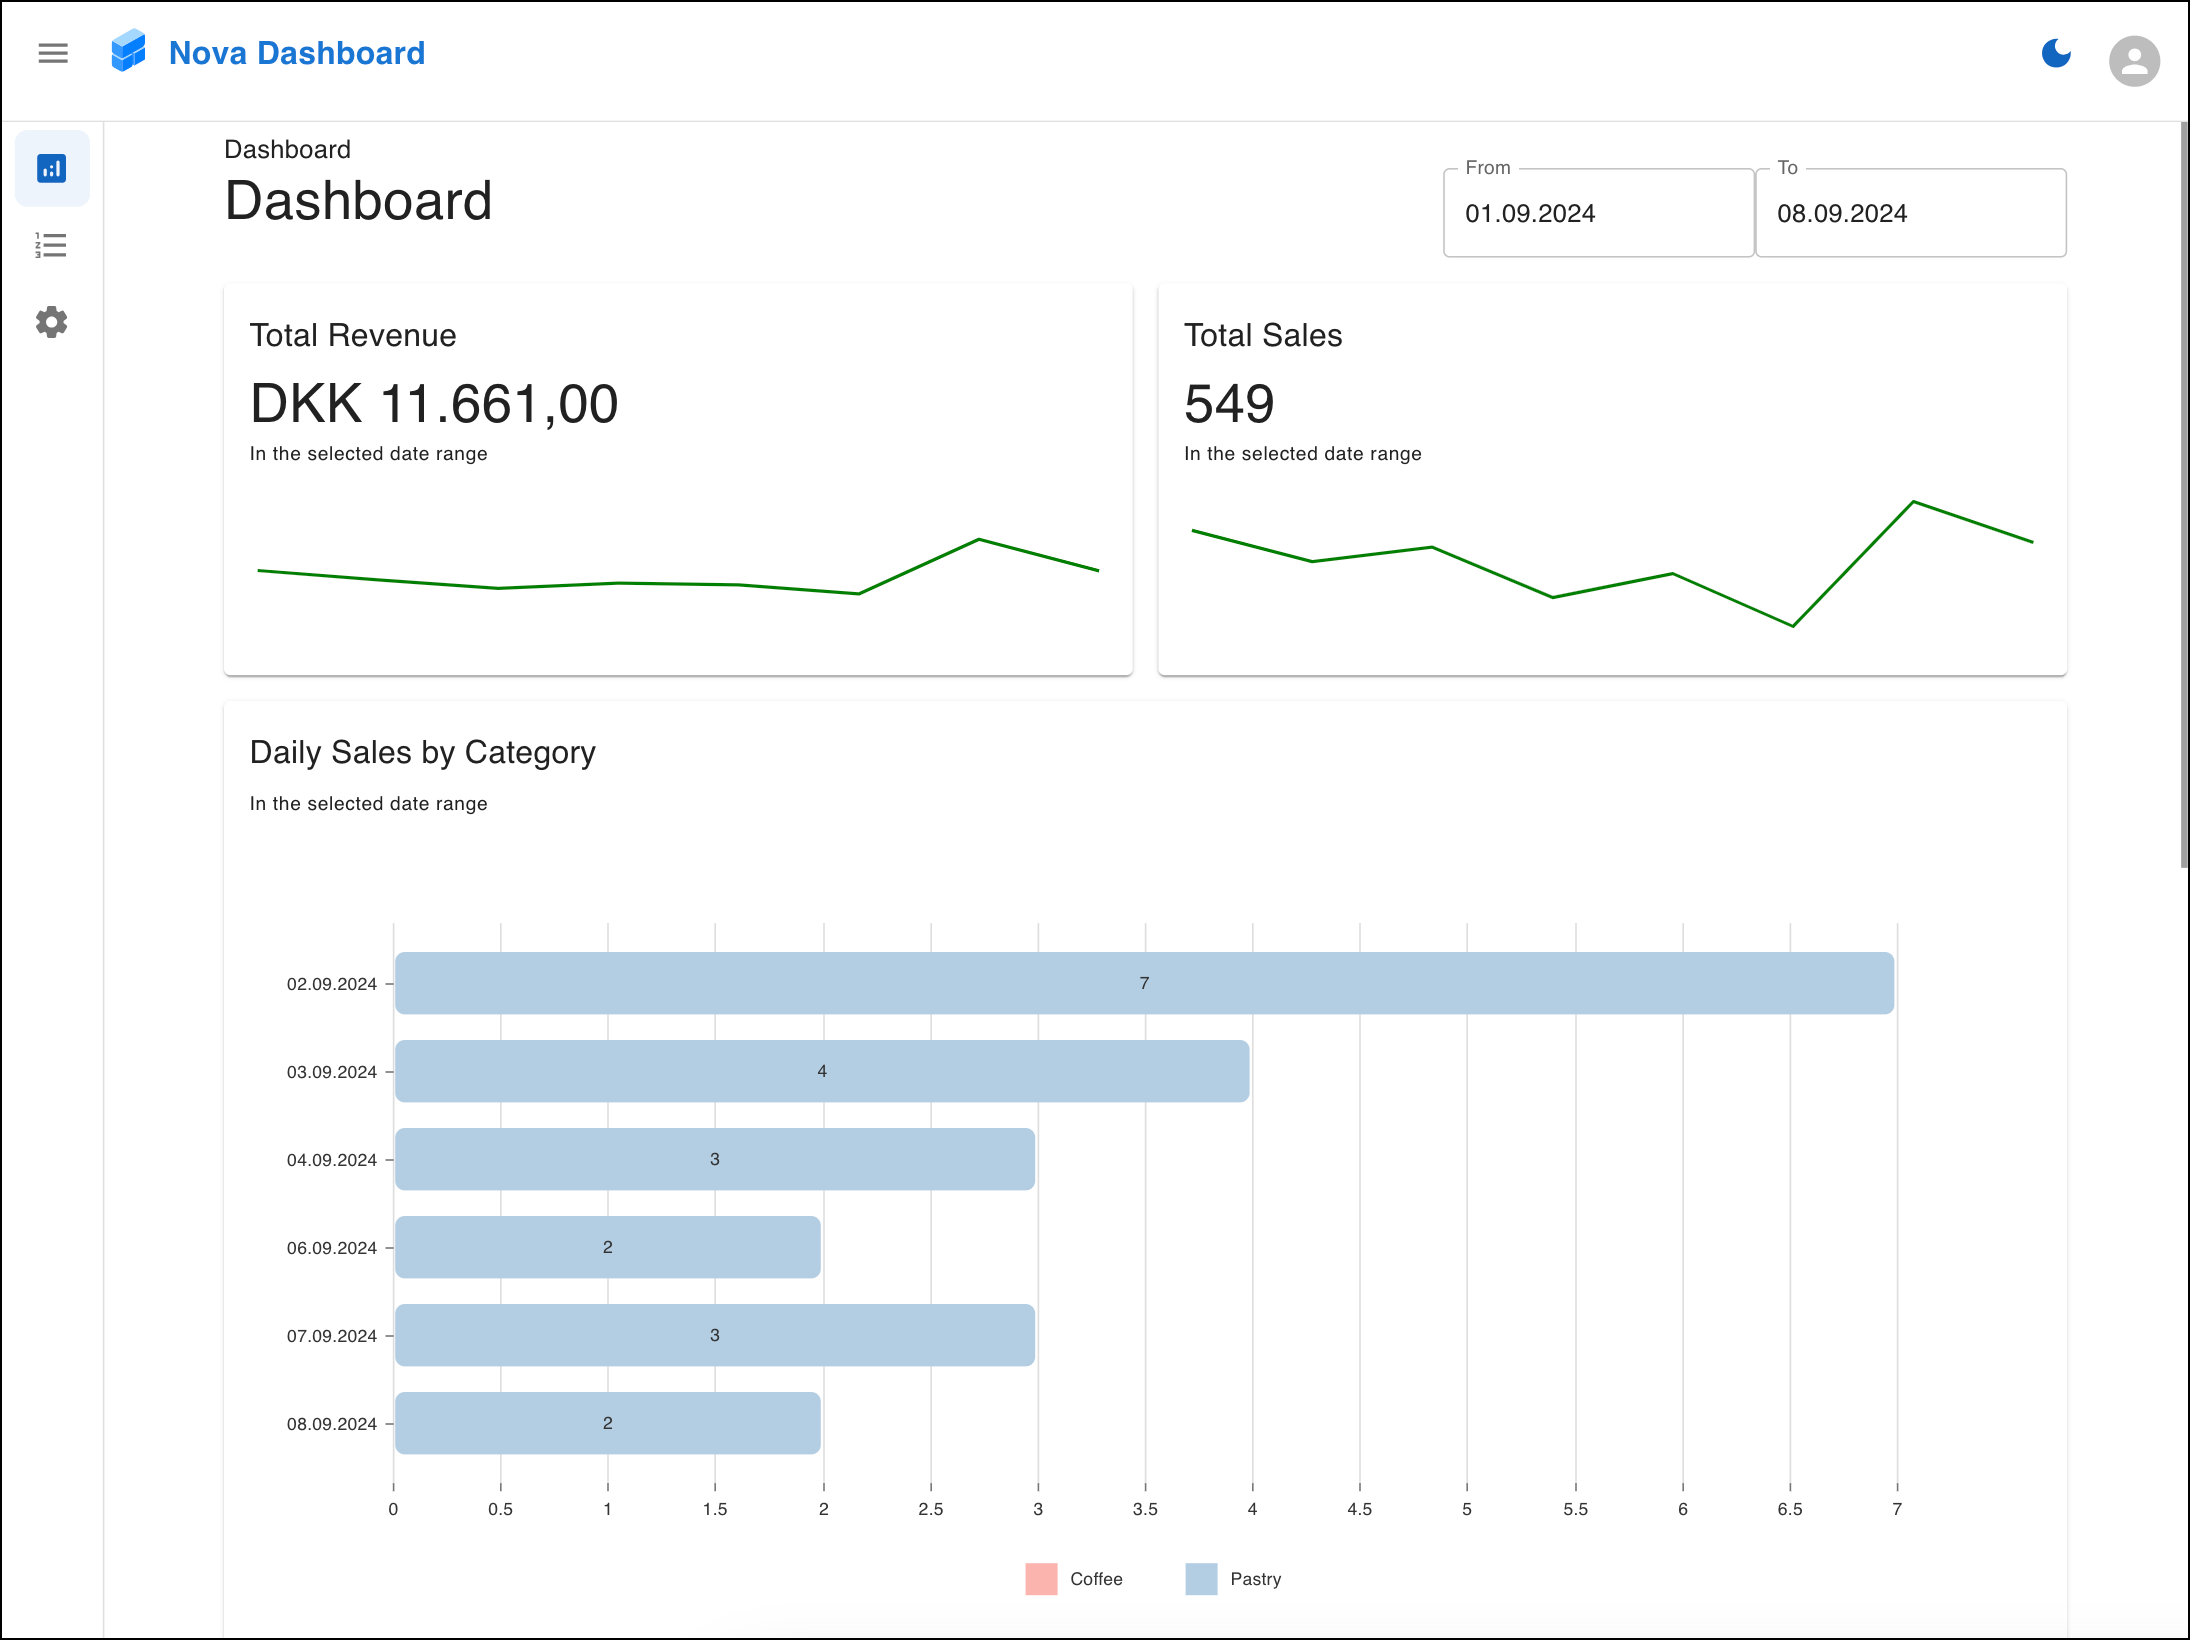
\includegraphics[width=.8\textwidth]{design-final-dash1.png}
    \caption{Final design of the dashboard, upper half.
    }\label{fig:design-final-dash1}
\end{figure}

\begin{figure}[H]
    \centering
    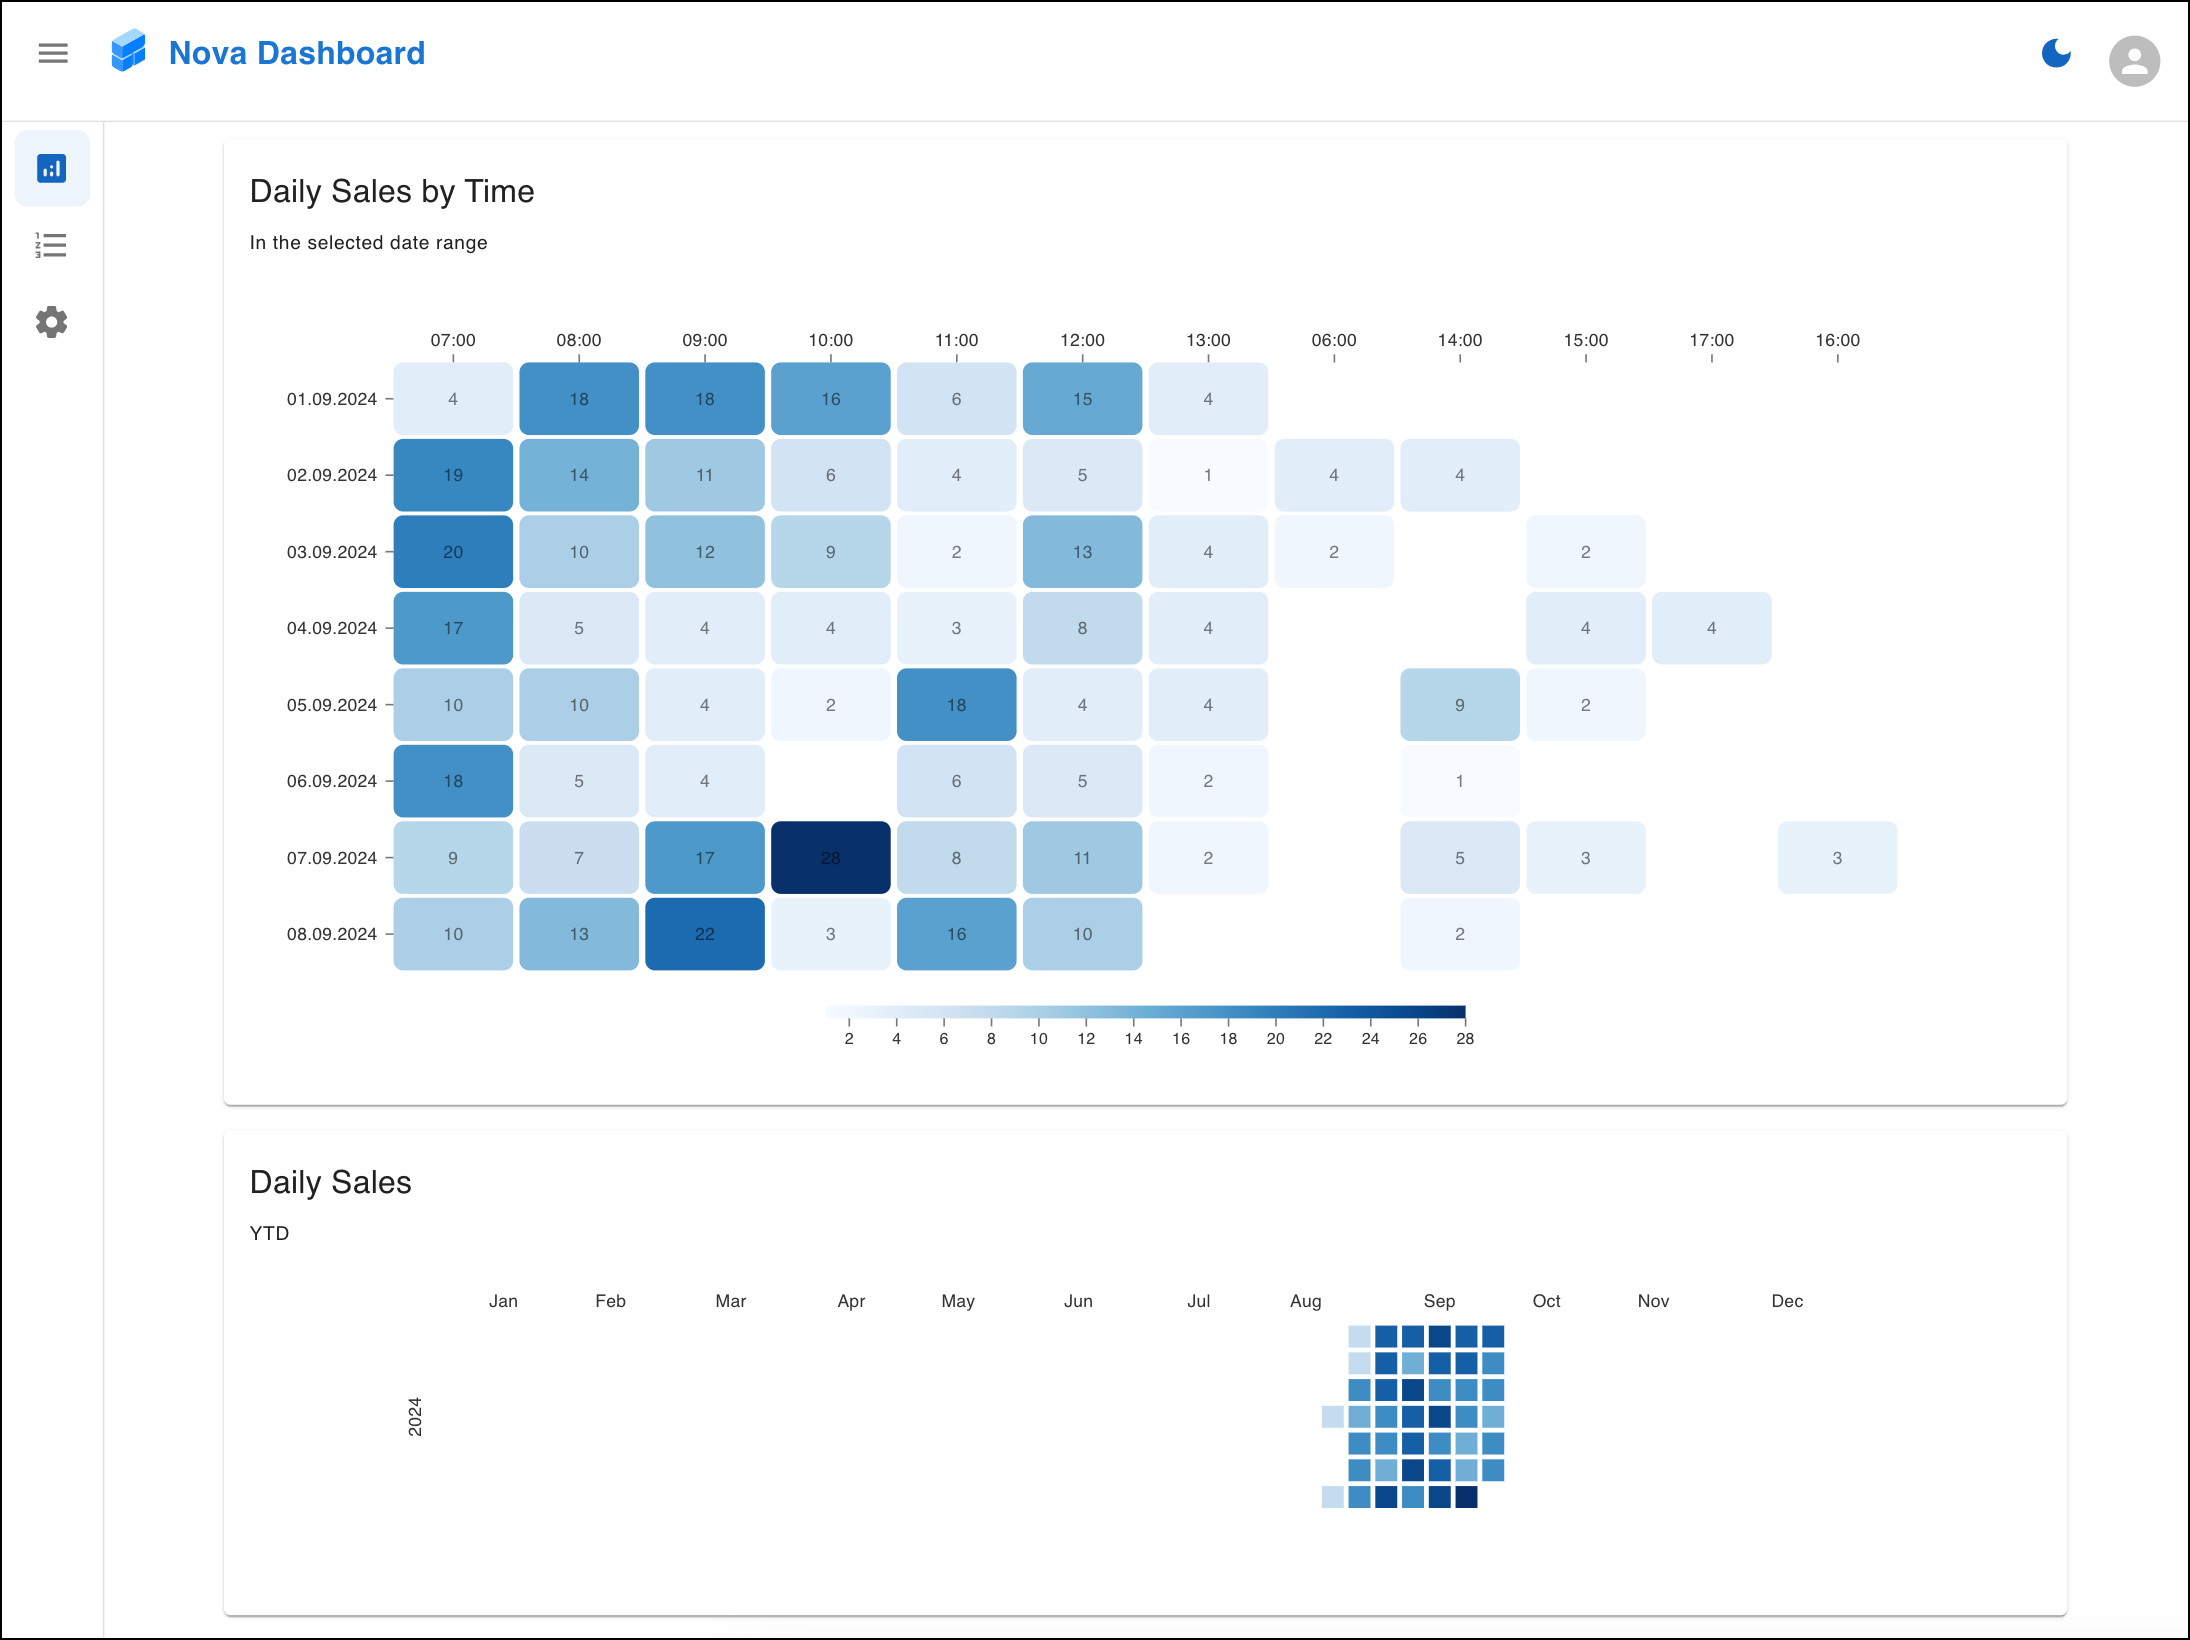
\includegraphics[width=.8\textwidth]{design-final-dash2.png}
    \caption{Final design of the dashboard, lower half.
    }\label{fig:design-final-dash2}
\end{figure}

More pages were added to the final design.
These pages deemed necessary for the application to be fully functional.
A settings page was added, where the upload buttons have been moved to.
This was done to clear up the dashboard and make it less cluttered.
The settings page also allow the user to create and assign categories to items.
The page can be seen in Figure~\ref{fig:design-final-settings} and the act or assigning categories can be seen in
Figure~\ref{fig:design-final-categories}.
Upon successful data upload request, a notification will appear on the bottom left of the screen, as seen in
Figure~\ref{fig:design-final-notification}.

\begin{figure}[H]
    \centering
    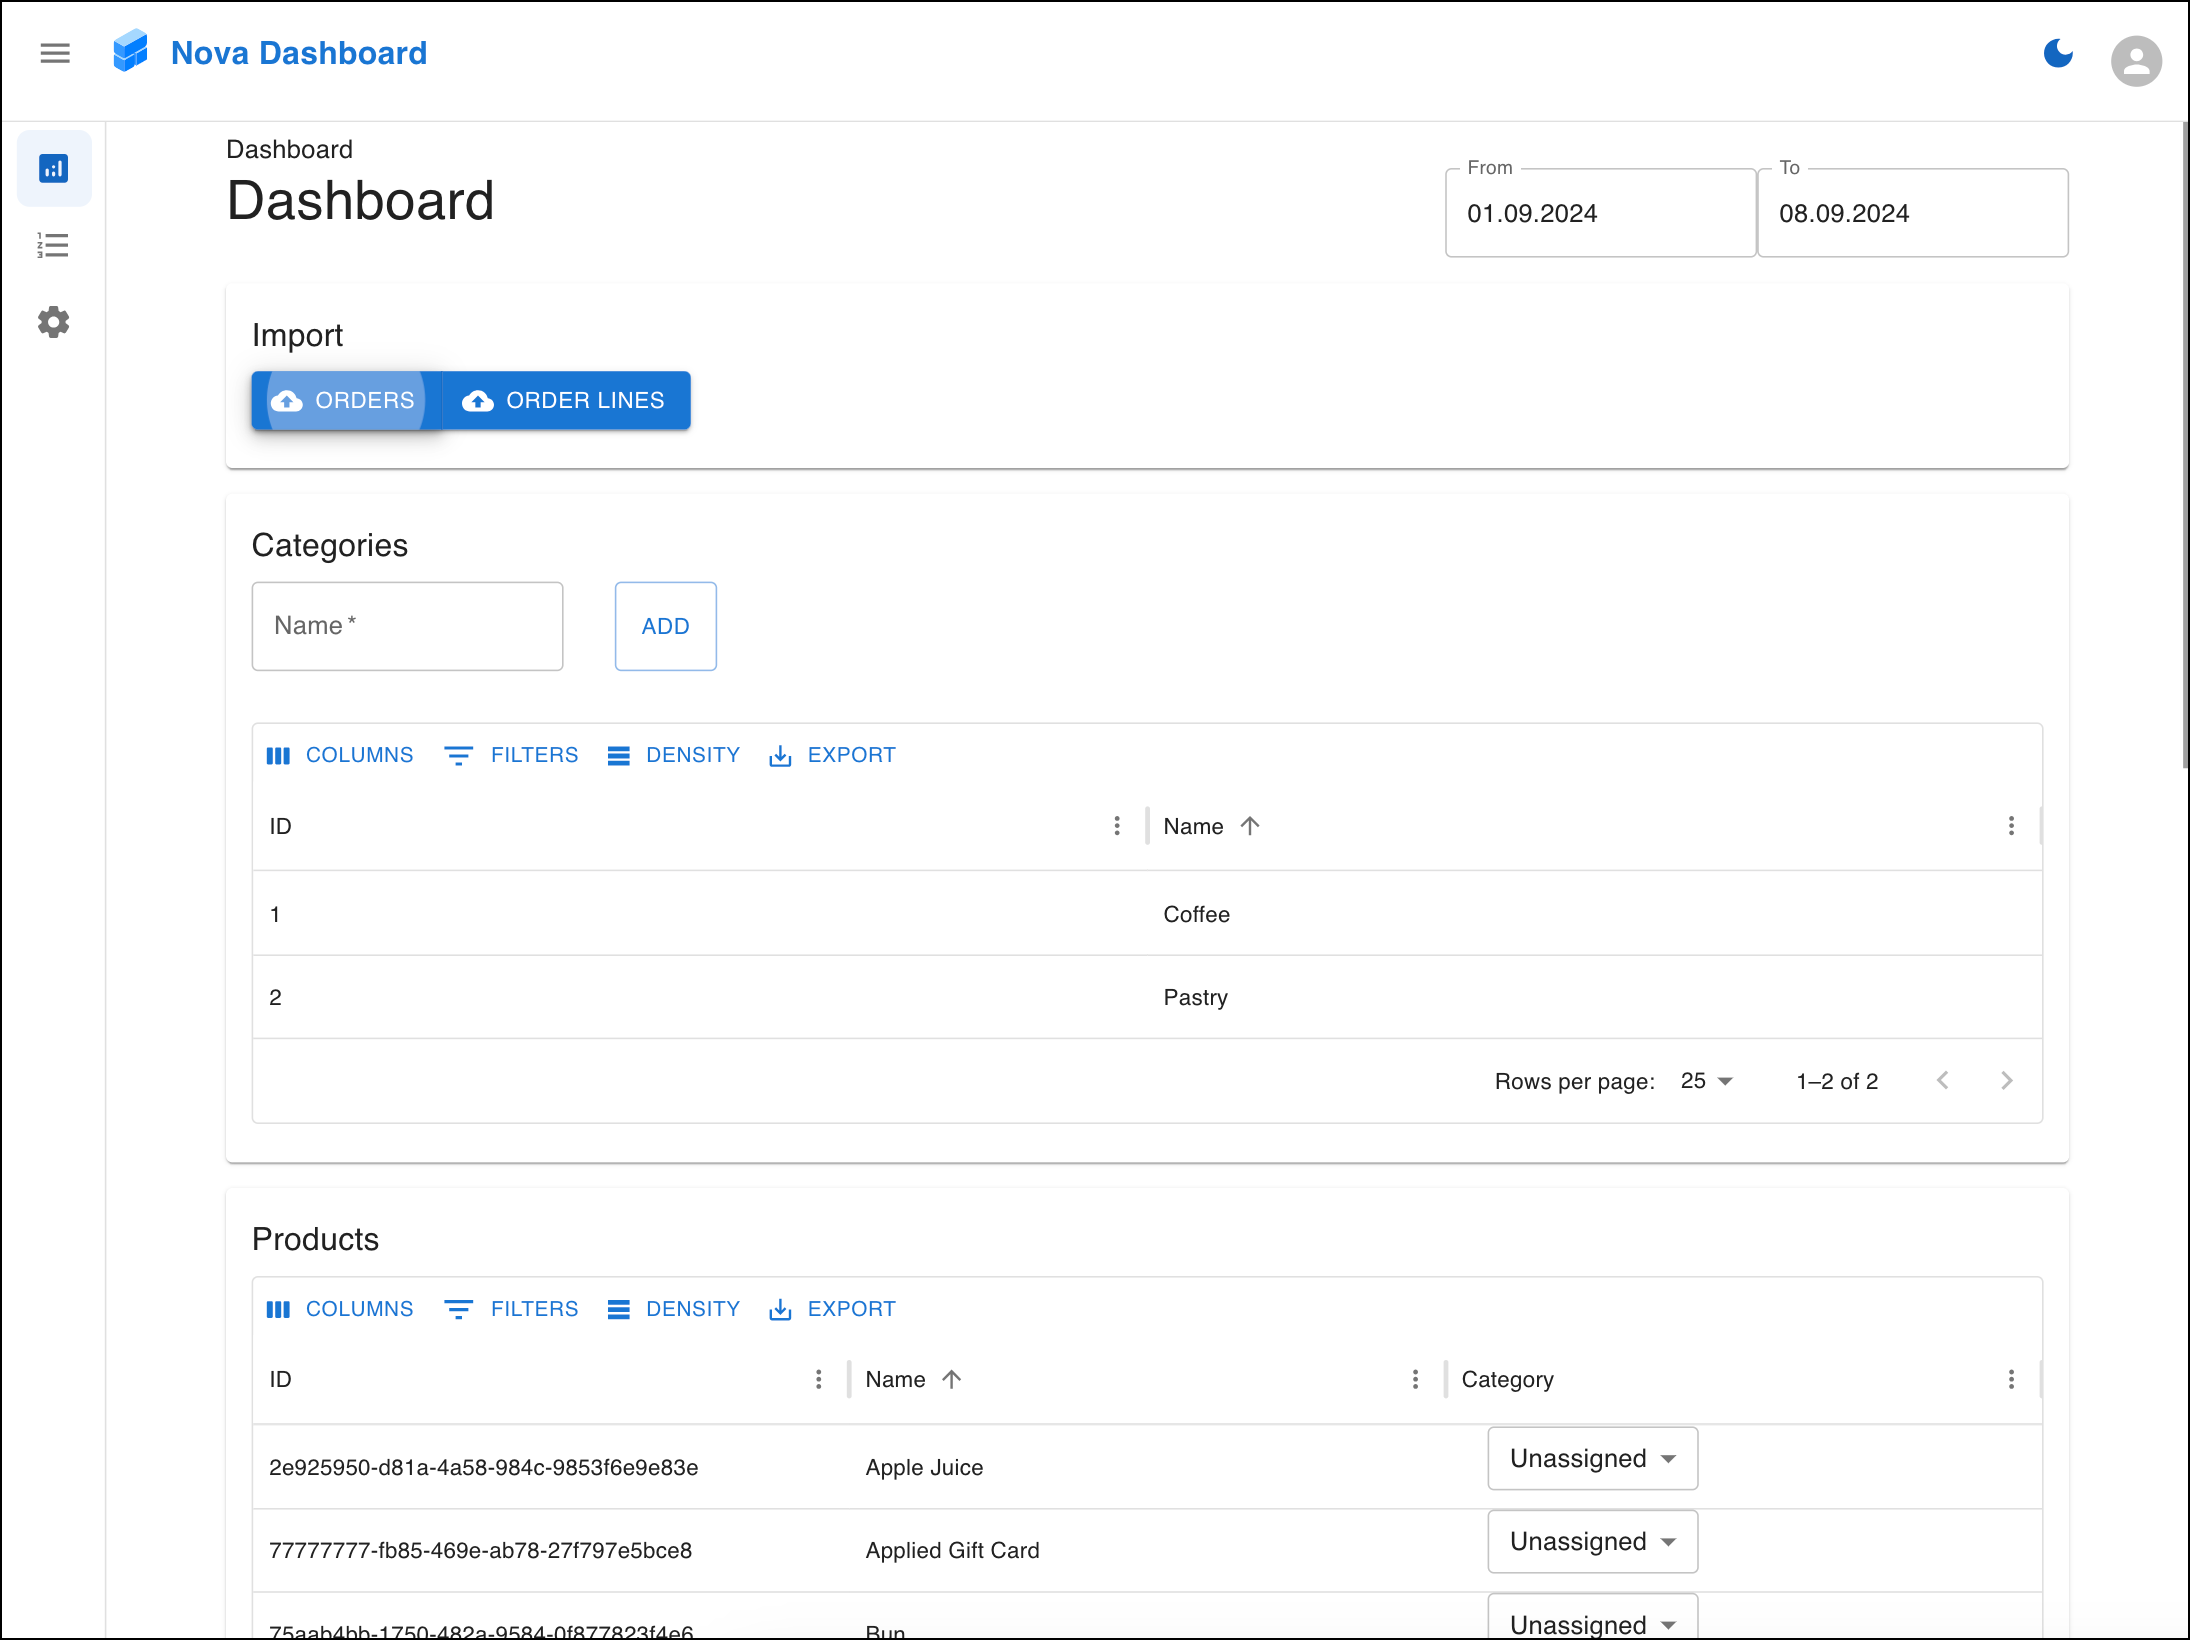
\includegraphics[width=.8\textwidth]{design-final-settings.png}
    \caption{Final design of the settings screen.
    }\label{fig:design-final-settings}
\end{figure}

\begin{figure}[H]
    \centering
    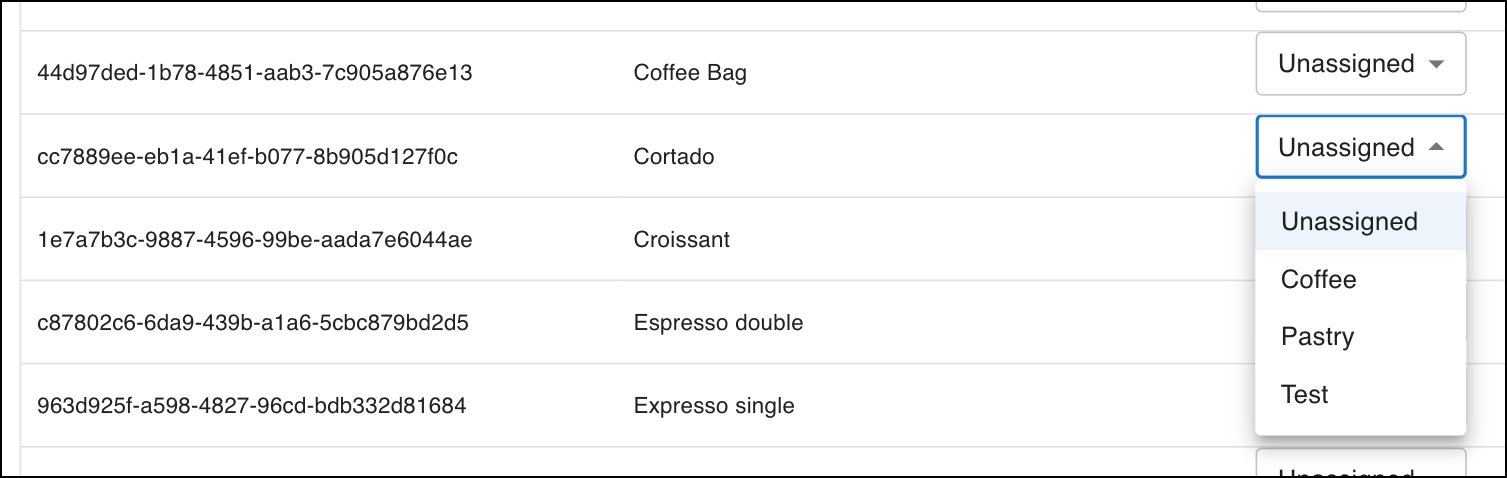
\includegraphics[width=.7\textwidth]{design-final-categories.png}
    \caption{Attaching categories to items.
    }\label{fig:design-final-categories}
\end{figure}

\begin{figure}[H]
    \centering
    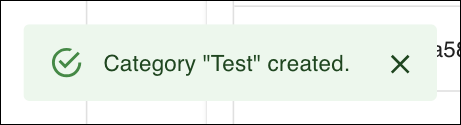
\includegraphics[width=.3\textwidth]{design-final-notification.png}
    \caption{Notification upon successful data upload request.
    }\label{fig:design-final-notification}
\end{figure}

The last page that was added is the sales page.
This page shows a list of all sales that have been made as raw data.
The page can be seen in Figure~\ref{fig:design-final-sales}.

\begin{figure}[H]
    \centering
    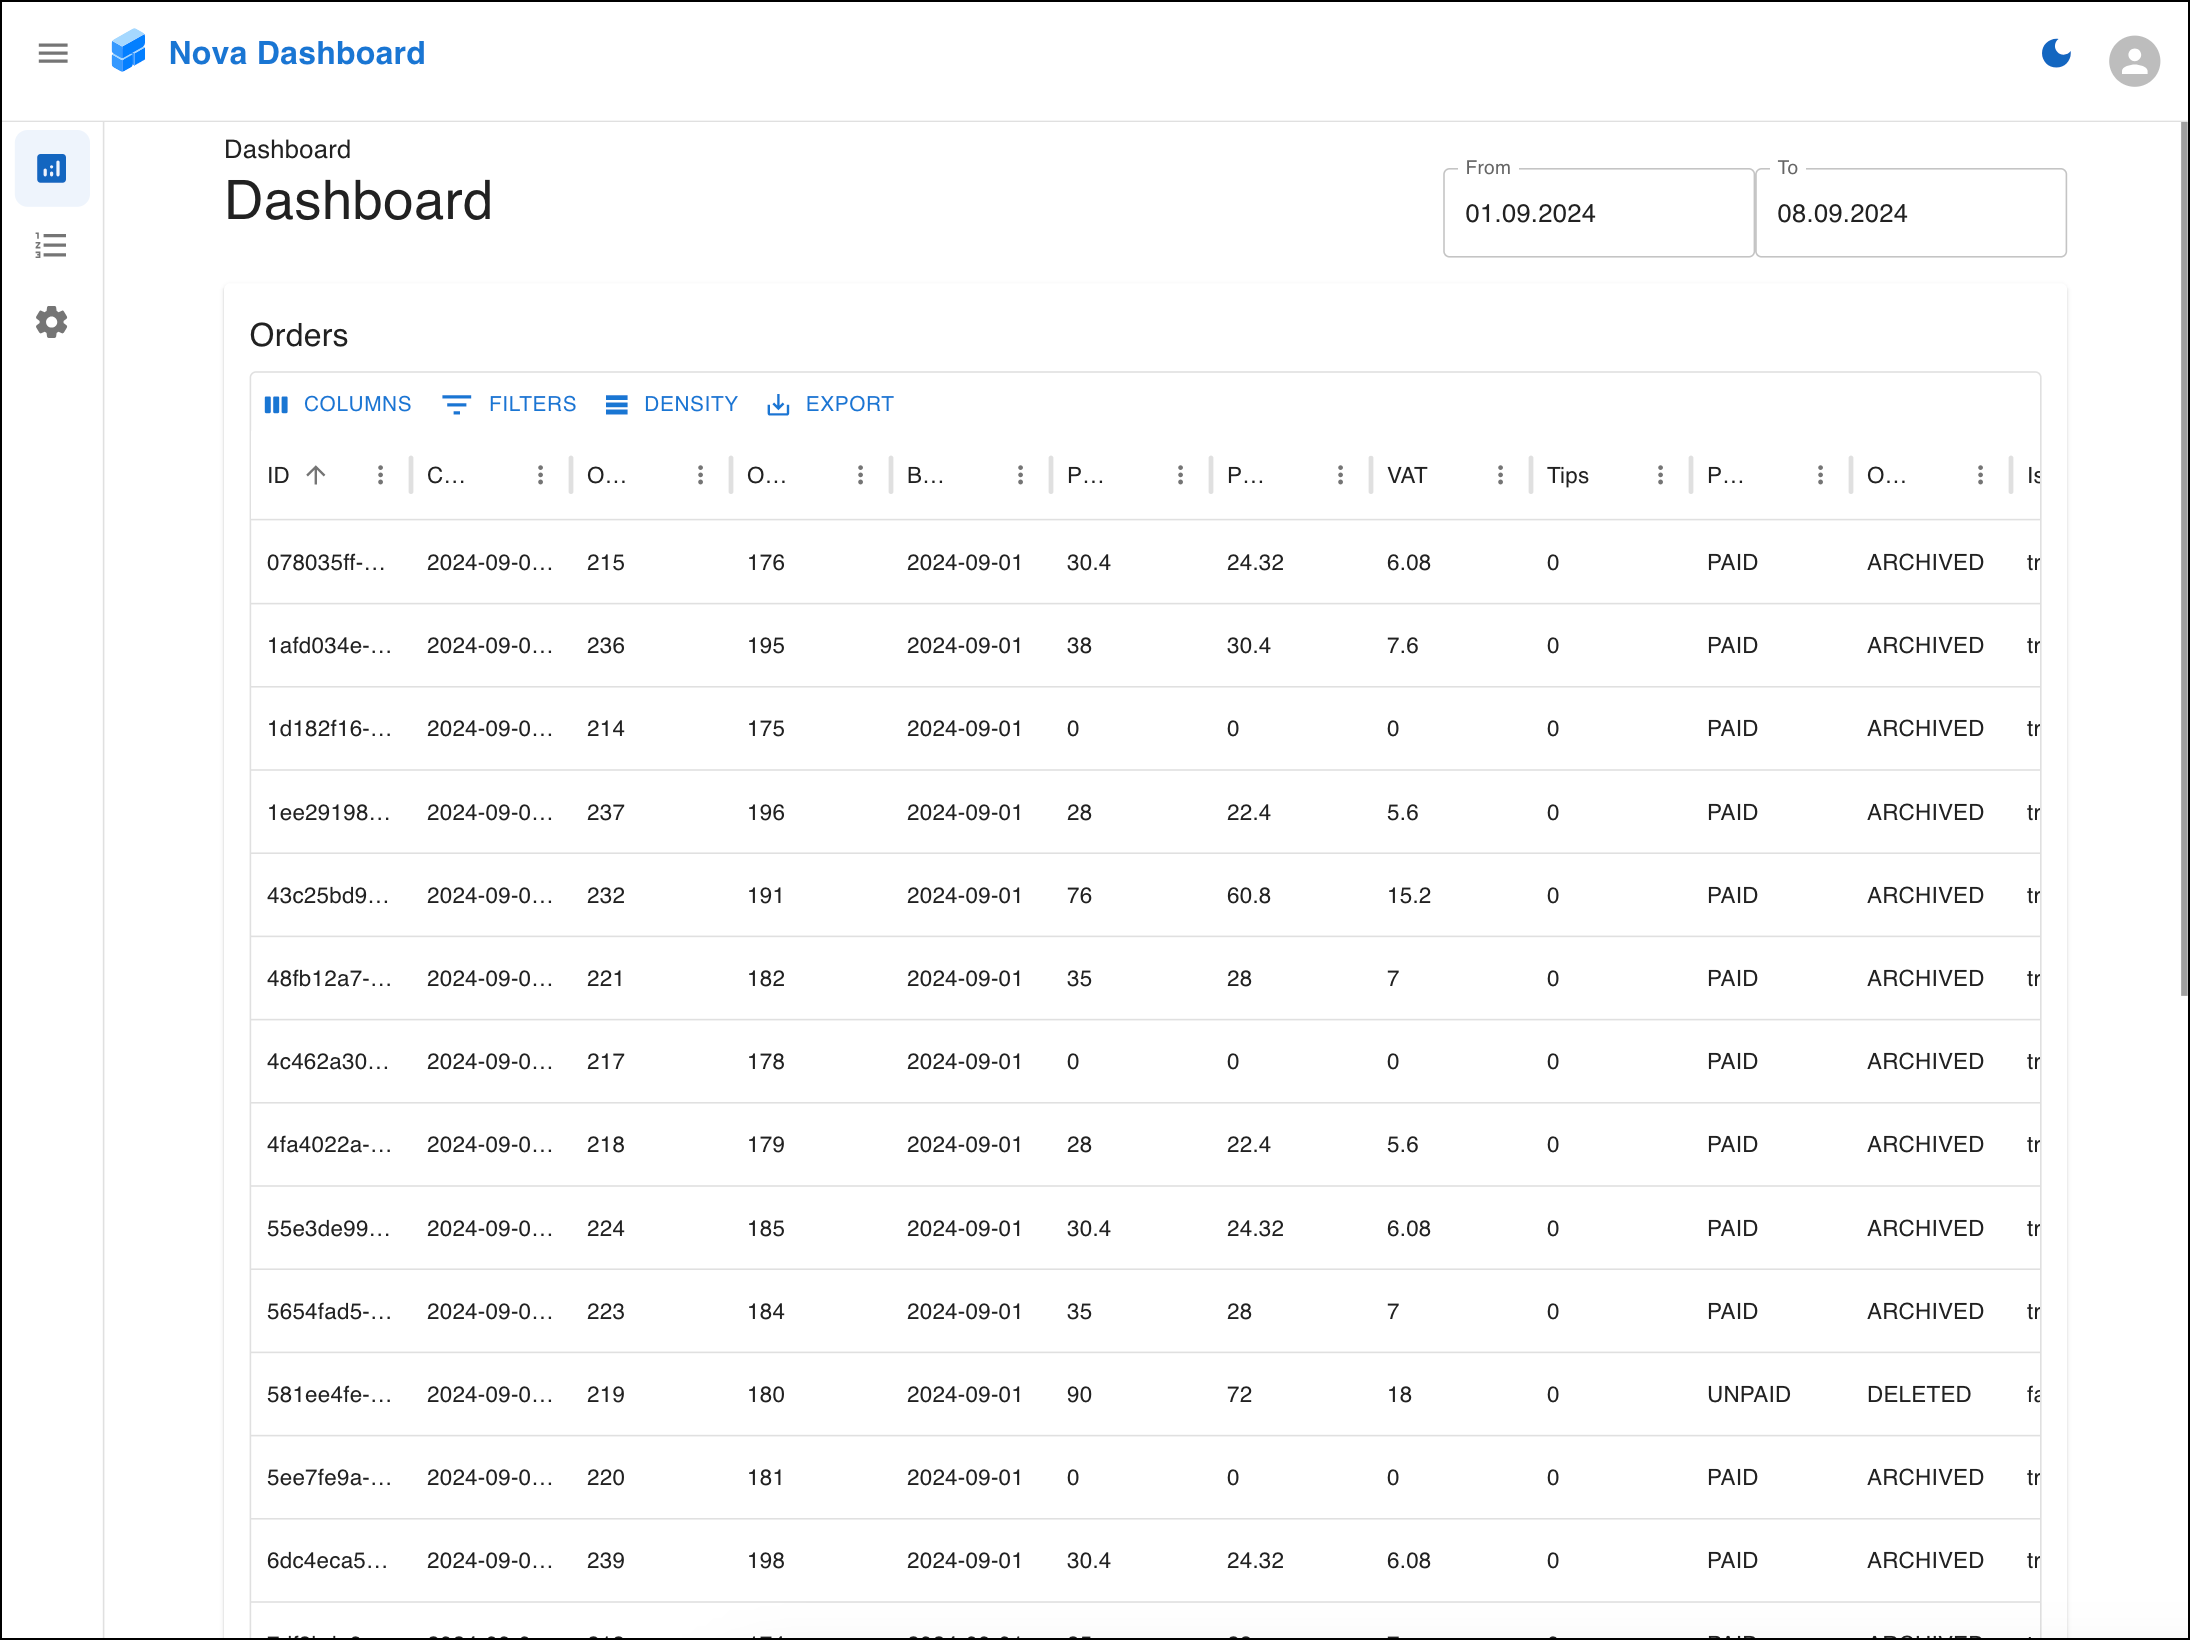
\includegraphics[width=.8\textwidth]{design-final-sales.png}
    \caption{Final design showing the full list of sales.
    }\label{fig:design-final-sales}
\end{figure}

Several functionalities were added to improve the user experience.
Most notably, the group added a functional filter to the dashboard.
There are two buttons on the top right of the dashboard that allows the user to filter the data by entering a specific
date range.
The date picker can be seen in Figure~\ref{fig:design-final-filter}.

\begin{figure}[H]
    \centering
    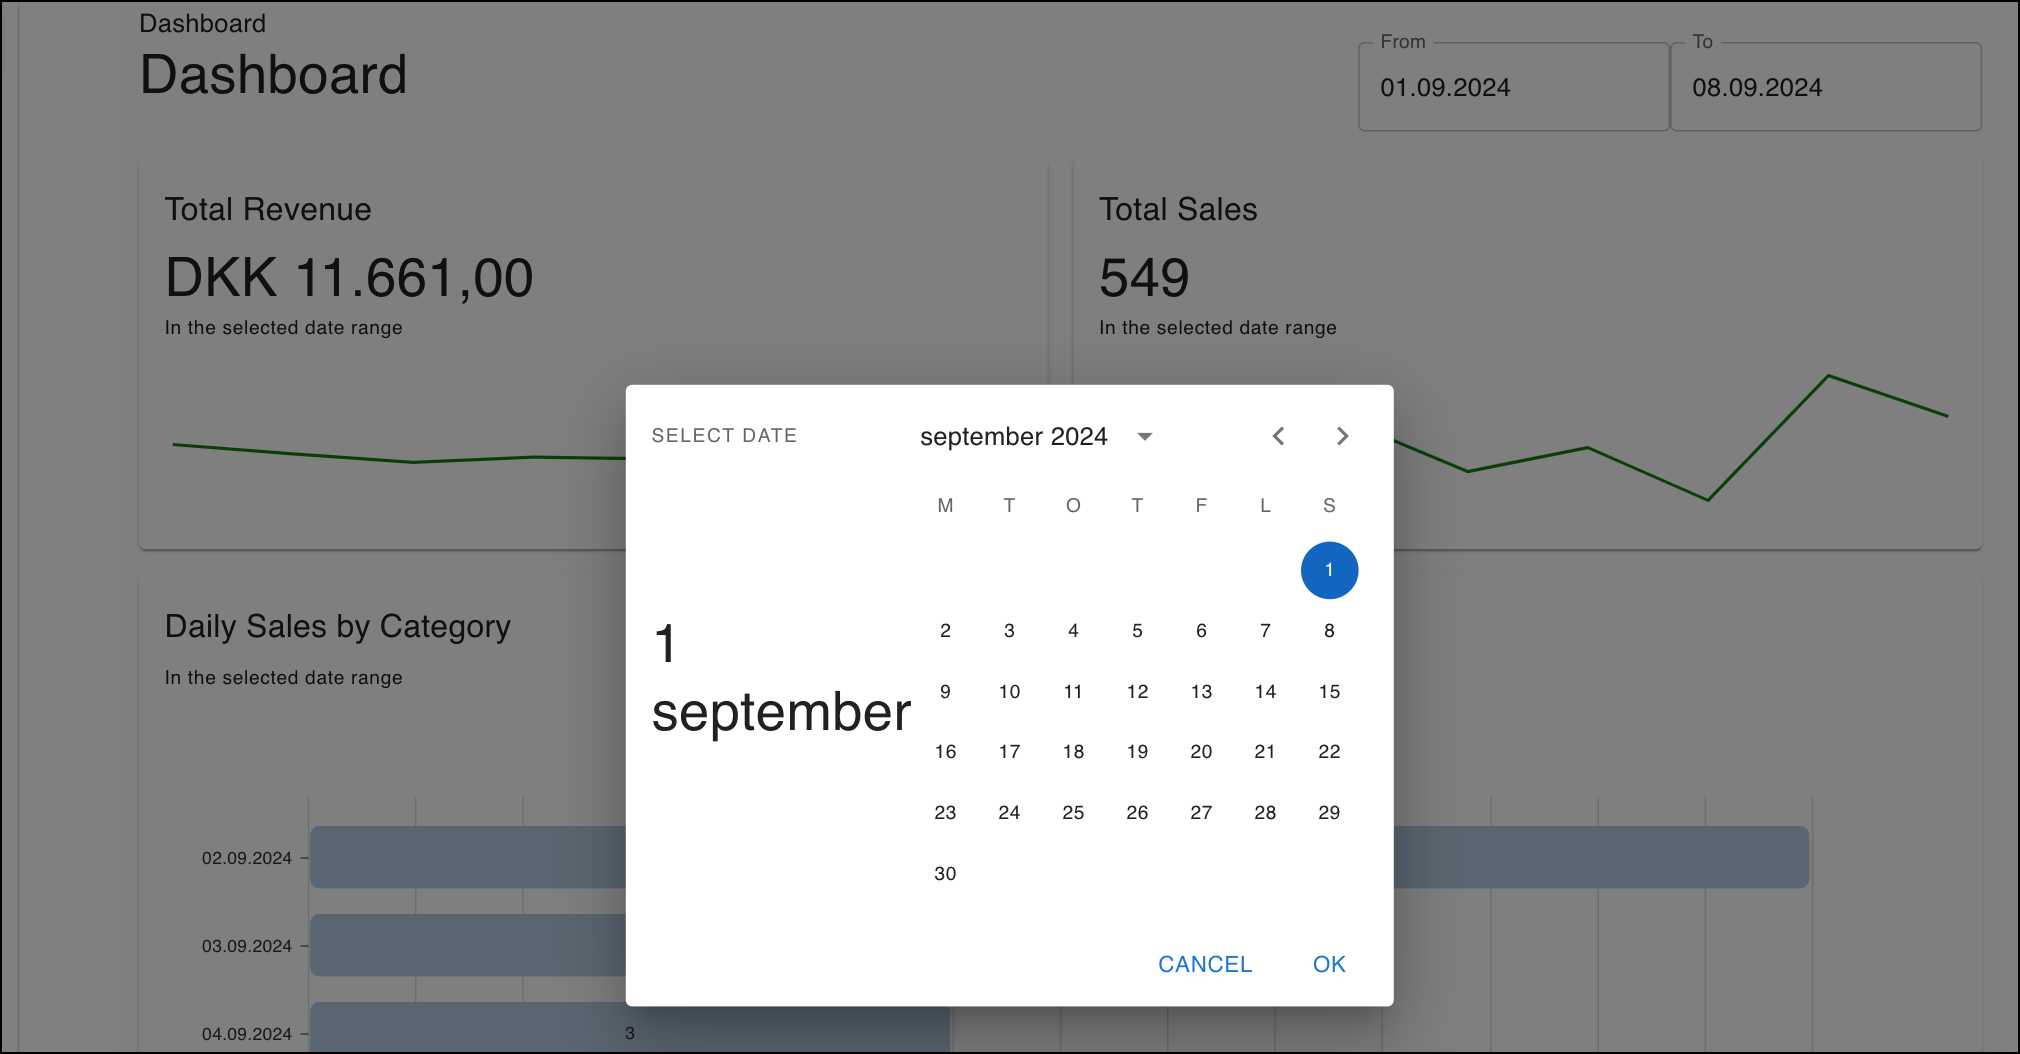
\includegraphics[width=.7\textwidth]{design-final-filter.png}
    \caption{Data filtering using a calendar.
    }\label{fig:design-final-filter}
\end{figure}

Lastly, to improve the usability on a tablet, the navigation bar was moved from the top to the side of the page.
This allows for more vertical space for the charts.
The navigation bar is collapsible, and the user can expand it by clicking the hamburger menu.
This was again done to allow for more space for the charts.
The prior charts show the collapsed navigation bar, and the expanded navigation bar can be seen in
Figure~\ref{fig:design-final-menu}.

\begin{figure}[H]
    \centering
    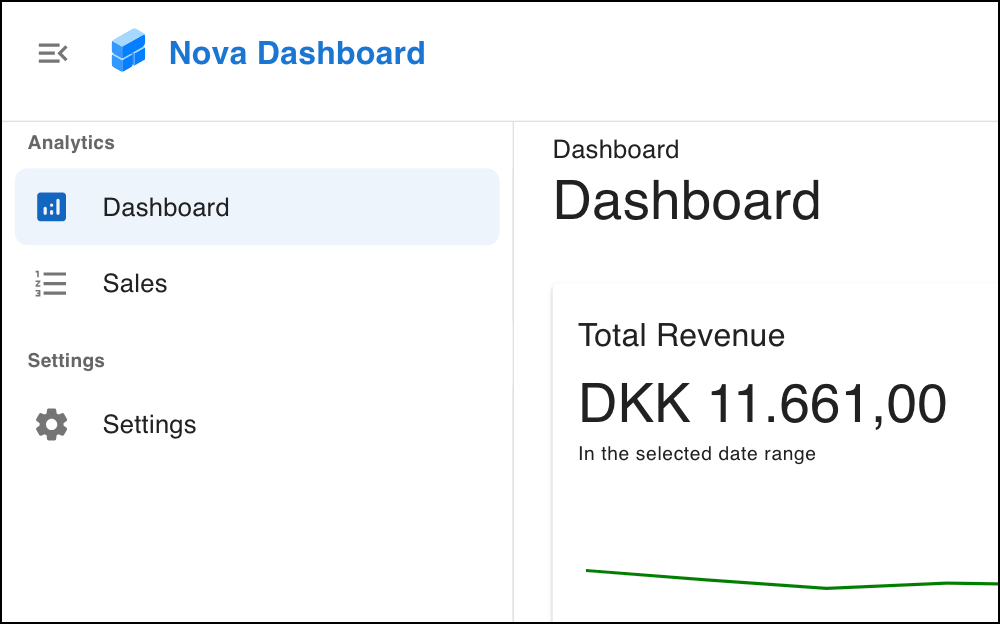
\includegraphics[width=.4\textwidth]{design-final-menu.png}
    \caption{Expanded hamburger menu.
    }\label{fig:design-final-menu}
\end{figure}
